\section{NAOqi Framework}

NAOqi ist der Name der Software, die tatsächlich auf dem Roboter läuft und ihn kontrolliert. Das NAOqi Framework ist das Gerüst, um Nao zu programmieren. Es spricht auf die gewöhnlichen Anforderungen in der Robotertechnik an: Parallelität (von Threads), Ressourcen, Synchronisation und Events. Das bedeutet, es kann mit allen gängigen Techniken der Software-Entwicklung bedient werden. 

Dieses Framework erlaubt homogene Kommunikation zwischen verschiedenen Modulen (Bewegung, Audio, Video), homogene Programmierung und homogenes Teilen von Informationen über die verschiedenen Module hinweg.
\\
\\
\noindent
Bild \myref{f:naoqi_ov} zeigt die einzelnen Komponenten des NAOqi Frameworks:
\begin{itemize}
\item Cross-Plattform
\item Cross-Language
\item NAOqi-Prozess
\item Module
\end{itemize}

\begin{figure}[H]						
	\centering							
	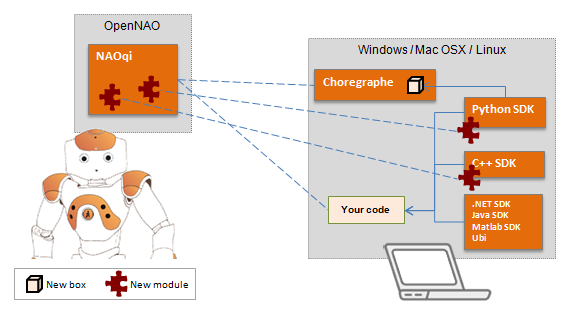
\includegraphics[scale=0.8]{Bilder/naoqi_ov.PNG}
	\caption{NAOqi Übersicht}						
	\label{f:naoqi_ov}						
\end{figure}


\subsection{Cross-Plattform/Language}

\textbf{Cross-Plattform}
\\
Cross-Plattform bedeutet Plattformunabhängigkeit gegenüber dem Betriebssystem auf dem programmiert werden soll. Sowohl auf Linux, Windows und auf Mac kann Code für Nao entwickelt werden. Allerdings kann auf Windows und Mac nur Code auf dem Computer kompiliert werden, während auf Linux der Code auch auf dem Roboter selbst übersetzt werden kann.
\\
\\
\textbf{Cross-Language}
\\	
Cross-Language ist nach \cite{ws:naodocu} die Eigenschaft, dass Software in C++ und in Python entwickelt werden kann. In allen Fällen, in denen die Methoden exakt gleich sind, kann das \ac{API} (dt: Programmierschnittstelle), gleichgültig von welcher der unterstützten Programmiersprachen, aufgerufen werden. Die \ac{API} ist in acht Programmiersprachen verfügbar: C++, Python, .NET (C\#, Visual Basic, F\#), Java, Matlab und Urbi.

Neue NAOqi Module können nur in C++ oder Python entwickelt werden, jedoch kann die Client-API mit allen Programmiersprachen angesprochen werden. Ebenso sind nur C++ und Python auf dem Roboter unterstützt, die anderen Sprachen werden nur über \textit{Remote-Access} supported. (Siehe unten \textit{Proxy})
\\
\subsection{NAOqi-Prozess}
Der NAOqi-Prozess, der auf dem Roboter läuft, ist ein \textit{Broker} (Siehe unten). Beim Start des Prozesses wird eine Konfigurationsdatei \textsf{autoload.ini} geladen, die definiert, welche Bibliotheken geladen werden sollen. Jede Bibliothek beinhaltet ein oder mehrere Module, die der Broker nutzt, um deren Methoden öffentlich anzuzeigen (Siehe Abbildung \myref{f:naoqi_broker1}).

\begin{figure}[H]						
	\centering							
	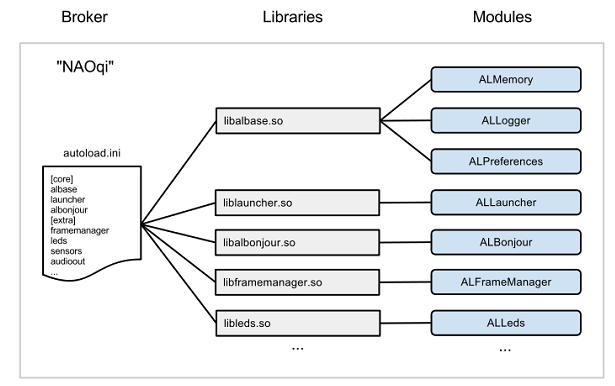
\includegraphics[scale=0.8]{Bilder/naoqi_process1.PNG}
	\caption{NAOqi Broker}						
	\label{f:naoqi_broker1}						
\end{figure}

Der Broker stellt einen Lookup-Service zur Verfügung, so dass jedes Modul im Baum oder verteilt im Netzwerk jede Methode finden kann, die öffentlich angezeigt wurde.

Das Laden der Module zum Start erzeugt einen Baum von Methoden, die an Module und diese wiederum an einen Broker geknüpft sind (Siehe Abbildung \myref{f:naoqi_broker2}).

\begin{figure}[H]						
	\centering							
	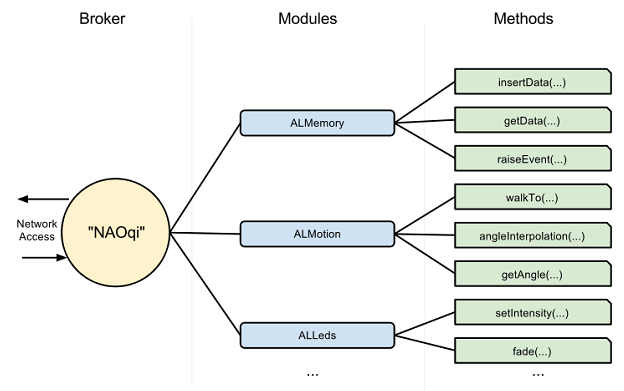
\includegraphics[scale=0.8]{Bilder/naoqi_process2.PNG}
	\caption{NAOqi Method-Tree}						
	\label{f:naoqi_broker2}						
\end{figure}
\noindent
\textbf{Broker}
\\
Der Broker ist ein Objekt, der zwei generelle Rollen einnimmt. Erstens ist es ein Verzeichnisdienst, mit dessen Hilfe Module und Methoden gefunden werden können und zweitens ein Netzwerk-Anschluss, der es möglich macht Methoden verknüpfter Module auch außerhalb des Prozesses aufzurufen.

Die meiste Zeit muss sich keine Gedanken um die Broker gemacht werden, da diese ihre Arbeit selbstständig und transparent erledigen. Geschriebener Code kann gleich sein, ob für Aufrufe an "`remote Modulen"' (dt.: entfernt; anderer Prozess oder anderes System) oder an "`lokalen Modulen"' (gleicher Prozess).
\\
\\
\textbf{Proxy}
\\
Ein Proxy ist ein Stellvertreterobjekt, das sich genau so verhält, wie das Modul das es repräsentiert. Wenn ein Proxyobjekt des ALMotion Moduls instanziiert wird, erhält das Proxyobjekt auch alle Methoden des \textsf{ALMotion} Moduls.
\newline
\newline
Um ein Proxy eines Moduls zu instanziieren, gibt es zwei Möglichkeiten: 
\begin{itemize}
\item Nur den Namen des Moduls benutzen. In diesem Fall muss der auszuführende Code und das Modul das verbunden werden soll im selben Broker liegen. Dies ist ein "`lokaler"' Aufruf
\item Zusätzlich zum Namen des Moduls auch die IP und den Port des Brokers benutzen. In diesem Fall muss das Modul im zugehörigen Broker liegen. Dies ist ein "`remote"' Aufruf.
\end{itemize}
Der genaue Unterschied zwischen "`remote"' und "`lokalen"' Modulen wird im Folgenden erklärt.
\\
\subsection{Module}
Typischerweise ist ein Modul eine Klasse innerhalb einer Bibliothek und wird automatisch instanziiert, wenn diese  durch \textsf{autoload.ini} geladen wird. Neue Methoden können an Klassen gebunden werden, die von \textsf{ALModule} erben. Dadurch werden die Methoden mit ihrem Namen und ihrer Signatur dem Broker öffentlich gemacht, so dass diese anderen verfügbar wird.
Ein Modul kann, wie oben bereits erwähnt, entweder "`remote"' oder "`lokal"' sein. 

\textbf{Lokale Module } sind zwei (oder mehr) Module, die im selben Prozess gestartet wurden. Sie kommunizieren miteinander lediglich über \textbf{einen} Broker. Durch den gemeinsamen Prozess können sie sich  Variablen teilen und einander Methoden ohne Serialisierung oder Netzwerkverbindung aufrufen. Dies erlaubt die schnellste Kommunikation untereinander. Lokale Module werden als Bibliothek kompiliert und können ausschließlich auf dem Roboter ausgeführt werden. Sie sind sehr schnell und effizient im Umgang mit dem Arbeitsspeicher.

\textbf{Remote Module} kommunizieren über das Netzwerk miteinander. Jedes remote Module benötigt einen Broker, um mit anderen Modulen zu sprechen. Der Broker nutzt dabei das Netzwerkprotokoll SOAP\footnote{Simple Object Access Protocol, dient u.a. dazu \textit{Remoe Procedure Calls} durchzuführen} zur Bereitstellung der Kommunikation. Schnelles Ansprechen von Modulen ist über ein remote Modul nicht möglich, beispielsweise bei direkter Adressierung des Arbeitsspeichers. Remote Module werden als ausführbare Dateien kompiliert und können außerhalb des Roboters aufgerufen werden. Remote Module sind einfacher zu benutzen und können dadurch von außen einfacher debuggt werden. Allerdings sind sie langsamer und weit weniger effizient wie lokale Module. 
\\
Die Kommunikation zwischen remote Modulen kann über zwei Wege erfolgen. Erstens \textbf{Broker to Broker} und zweitens \textbf{Proxy to Broker}.
 
Der Unterschied liegt darin, dass Broker to Broker eine wechselseitige, Proxy to Broker nur eine einseitige Kommunikation eröffnet. Bei zwei Modulen B und C kann bei Broker to Broker B Methoden von C und C Methoden von B aufrufen. Bei Proxy to Broker ist dies nur in die Richtung von B nach C möglich, nicht umgekehrt. Listing \ref{lst:module_comm} zeigt die Implementierung beider Kommunikationsarten.

\lstinputlisting
    [caption={Kommunikationsarten Module},
       label=lst:module_comm,
       captionpos=b]	
 {Listings/module_comm.cs}
\vspace{0.4cm}
\noindent	
\textbf{Blocking und non-Blocking Aufrufe}
\\
Das NAOqi-Framework bietet zwei Möglichkeiten an, Methoden aufzurufen. 
Abbildung \ref{f:naoqi_blockingcall} zeigt das Schema eines \textbf{Blocking calls}. Diese sind wie normale Methodenaufrufe. Die nächste Anweisung wird erst nach dem Ende der vorherigen ausgeführt und währenddessen ist keine Ausführung von anderem Code möglich. Alle Aufrufe können eine Exception auslösen und sollten in einen try-catch - Block gepackt werden. Ebenso können die Aufrufe Rückgabewerte besitzen.
\begin{figure}[H]						
	\centering							
	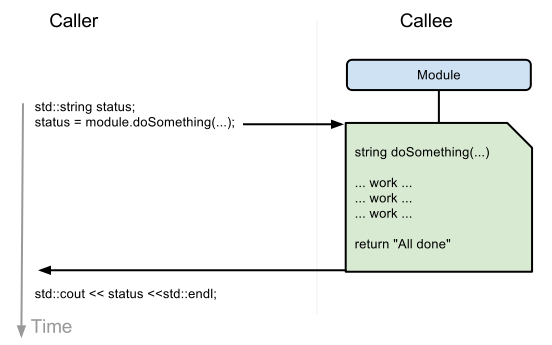
\includegraphics[scale=0.8]{Bilder/blockingcall.PNG}
	\caption{Blocking Call}						
	\label{f:naoqi_blockingcall}						
\end{figure}
\noindent
\textbf{Non-blocking calls} benutzen das \textit{post-}Objekt einer Proxy. Der Vergleich zu Abbildung \ref{f:naoqi_nonblockingcall} zeigt, dass die Ausführung der Methode in einen parallelen Thread gepackt wird. Dadurch ist es möglich, andere Anweisungen zur gleichen Zeit auszuführen, z.B. Sprechen während des Laufens. Jedes post-Objekt erzeugt eine \textit{taskID}. Mit dieser ID kann entweder geprüft werden ob der Thread noch läuft, ob auf ihn gewartet oder ob er gestoppt werden soll. 
\begin{figure}[H]						
	\centering							
	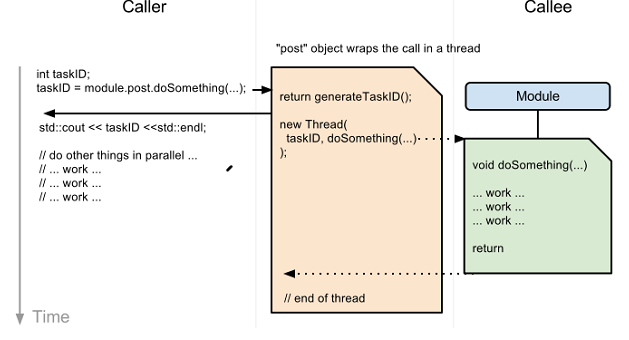
\includegraphics[scale=0.8]{Bilder/nonblockingcall.PNG}
	\caption{Non - Blocking Call}						
	\label{f:naoqi_nonblockingcall}						
\end{figure}


\subsection{.NET SDK}
Wie bereits in Kapitel \myref{Einleitung} erwähnt, wurde als Programmiersprache C\# gewählt. 
\\
Das Benutzen des .NET SDK ist sehr einfach gestaltet. Dazu muss dieses je nach .NET - Version (2/4) installiert werden. In unserem Fall ist das .NET Version 4, da mit \textit{Microsoft Visual Studio 2013} entwickelt wurde. Das SDK beinhaltet Auto-Vervollständigung und nahezu jede NAOqi-Methode kann damit aufgerufen werden.
\\
 Listing \ref{lst:net_helloWorld} zeigt ein einfaches Beispiel zur Benutzung von NAOqi innerhalb C\#. In Zeile eins wird angegeben, dass der Namespace von NAOqi benutzt wird. Damit dies möglich ist, muss davor die \textsf{naoqi.dll} als Verweis dem Projekt hinzugefügt werden. Zeile sieben zeigt die Erzeugung eines Proxyobjekts vom Typ \textit{TextToSpeech}. Da im Konstruktor eine IP-Adresse und ein Port angegeben wird, handelt es sich hier um eine Proxy to Broker Kommunikation. Auf dem Proxyobjekt wird in Zeile acht eine Methode mit dem Parameter \textsf{"Hello World"} als blocking call aufgerufen. Das Ergebnis der Methode ist die sprachliche Ausgabe des Strings \textsf{Hello World} durch den Roboter.

\lstinputlisting
    [caption={Beispiel .NET SDK},captionpos=b,
       label=lst:net_helloWorld,
       ]	
 {Listings/helloWorld.cs}

